%
% LaTeX Report Assignment 4
% Applied Programming Lab EE2703
% Ayush Jamdar EE20B018 
%


\documentclass[11pt, a4paper]{article}
\usepackage{graphicx}
\usepackage{amsmath}
\usepackage{listings}
\usepackage[]{courier}
%\usepackage{hyperref}


\title{Assignment 5: The Resistor Problem} % Title

\author{Ayush Jamdar EE20B018} % Author name

\date{\today} % Date for the report
\begin{document}		
		
\maketitle % Insert the title, author and date
\section{Aim}
%Create new section;it is autonumbered
The goal is to solve for currents in a resistor. The currents depend on the shape of the resistor.
We work with a square plate of dimensions $1 cm$ by $1 cm$. 


\section{The Assignment}
On solving the Poissons's equation 
$$\nabla ^2\phi = 0$$
for the square plate we learned that potential at any point $(i, j)$ is the average of potential of its neighboring points.
Mathematically, it is stated as 
$$\phi_{i,j} = \frac{\phi_{i+1,j}+\phi_{i-1,j}+\phi_{i,j+1}+\phi_{i,j-1}}{4}$$
We'll use this result in the following analysis.

\section{Code}
\subsection{Libraries}
Required libraries are imported. 
\begin{verbatim}
from sys import argv, exit
import mpl_toolkits.mplot3d.axes3d as p3
from matplotlib.pyplot import *
import argparse
import numpy as np
\end{verbatim}

\subsection{Defining parameters}
First, let's define the plate axes. The square plate has the ground terminal connected along its lower horizontal edge and the central lead of 1 V is a disc of radius \texttt{radius}. Note that the code is also designed to work for unequal values of \texttt{Nx} and \texttt{Ny}. 

\begin{figure}[!tbh]
   	\centering
  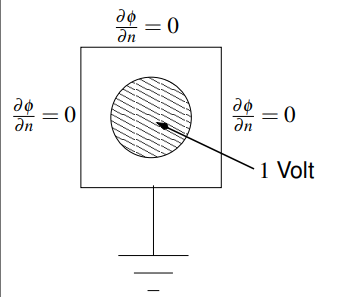
\includegraphics[scale=0.5]{plate.png} 
    \caption{The Copper Plate} 	\label{The Plate}
   \end{figure} 

\texttt{Nx, Ny} are the number points along x and y, the potential of which is going to be analysed. \texttt{Nx = 25} and \texttt{Ny = 30} means I mark 25 points along the x-axis and 30 along the y and calculate potential at each of the points on the grid. We perform a number of iterations of the main algorithm to reach near accurate answers. This number is given by \texttt{Niter}. All of these three parameters can be given as commandline arguments using the form \texttt{python3 a5.py --Nx 26 --Ny 26 --radius 8 --Niter 3000
}. Otherwise the default values are \texttt{Nx = 25, Ny = 25, radius = 8, Niter = 1500}. 
But to do the commandline action, I have used a special library \texttt{argparse}. How it does the parsing is by the code below. (Reference {https://docs.python.org/3/library/argparse.html}) 
\begin{verbatim}
parser = argparse.ArgumentParser(
description='Processing plate data and number of iterations')
parser.add_argument('--Nx', type=int,
 default=25, help='size of plate along x')
parser.add_argument('--Ny', type=int,
 default=25, help='size of plate along y')
parser.add_argument('--radius', type=int,
 default=8, help='radius of central lead')
parser.add_argument('--Niter', type=int,
 default=1500, help='Number of iterations')
args = parser.parse_args()

Nx = args.Nx  # number of points taken along x in units
Ny = args.Ny  # number of points taken along y in units
radius = args.radius  # radius of central lead in units
Niter = args.Niter  # number of iterations to perform
\end{verbatim}

\subsection{Allocating the potential array}
Note that I'll go with the default values for further explanation. The potential matrix \texttt{phi} has \texttt{Ny} rows and \texttt{Nx} columns. The axes are marked such that the origin comes at the center of the plate. Hence the floor division and linspacing. 
\begin{verbatim}
phi = np.zeros((Ny, Nx))
x = np.linspace(-((Nx-1)//2), Nx//2, Nx)
y = np.linspace(-((Ny-1)//2), Ny//2, Ny)
X, Y = np.meshgrid(x, y)

ii = np.where(X**2 + Y**2 <= (radius**2))
\end{verbatim}

\texttt{meshgrid} returns two matrices \texttt{X} and \texttt{Y} which have the x and y coordinates of each of the points we mark on the plate. The \texttt{where} function returns the coordinates of those points which lie inside the radius of the central 1 V lead. Now what remains is just assigning 1 V potential to these points which is easily done by the line
\begin{verbatim}
phi[ii] = 1.0
\end{verbatim}  

A beautiful contour plot, Figure 2, born out of the following code,  illustrates the potential obtained so far.  

\begin{verbatim}
contourf(x, y, phi)  
colorbar()
scatter(X[ii], Y[ii], c='r', marker='o')
xlabel(r'x (plate dimension) $\rightarrow$')
ylabel(r'y (plate dimension) $\rightarrow$')
title("Contour plot of Potential")
show()
\end{verbatim}

\begin{figure}[!tbh]
   	\centering
  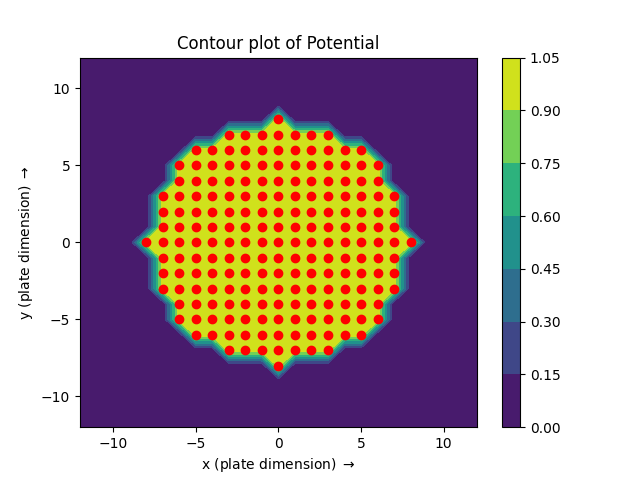
\includegraphics[scale=0.5]{Q1.png} 
    \caption{Potential Contour Plot}
   	\label{fig:contour potential)}
   \end{figure}
   
\subsection{Updating potential}
This is where the neighbour-average algorithm starts. In each of the \texttt{Niter} iterations, I update potential by taking this average. Simultaneously I measure the error or the maximum change in potential matrix occurring after that iteration. Instead of using nested \texttt{for} loops, a totally awesome way to do it is Python subarrays and vectorized code. The code also takes care of the boundary conditions - no current should flow out of the edges horizontally, zero potential on the bottom edge and 1 V on the center radius.

\begin{verbatim}
for k in range(Niter):
    oldphi = phi.copy()
    # using python subarrays
    left_neighbours = phi[1:-1, 0:-2]
    right_neighbours = phi[1:-1, 2:]
    top_neighbours = phi[0:-2, 1:-1]
    bottom_neighbours = phi[2:, 1:-1]
    phi[1:-1, 1:-1] = (left_neighbours+right_neighbours+
    top_neighbours+bottom_neighbours)/4

    # assert boudaries
    phi[1:-1, 0] = phi[1:-1, 1]  # left side
    phi[1:-1, -1] = phi[1:-1, -2]  # right side
    phi[0,1:-1] = phi[1, 1:-1]  # top
    phi[ii] = 1.0
    phi[-1, :] = 0  # ground at bottom edge
 
    errors[k] = (abs(phi - oldphi)).max()

\end{verbatim}
The most interesting part of this algorithm is the average calculation using subarrays. Potential at all the points is calculated in just one line and internally by C. A nested Python loop for the same would substantially raise the time complexity of the code. 

Two columns from the left and two from the right having the same potential implies that there is no potential gradient along the horizontal at the edges and hence no horizontal current. This is wonderfully done by a single line of code.
   
Now I plot the error and observe how error changes with each iteration in Figure 3.

\begin{figure}[!tbh]
   	\centering
  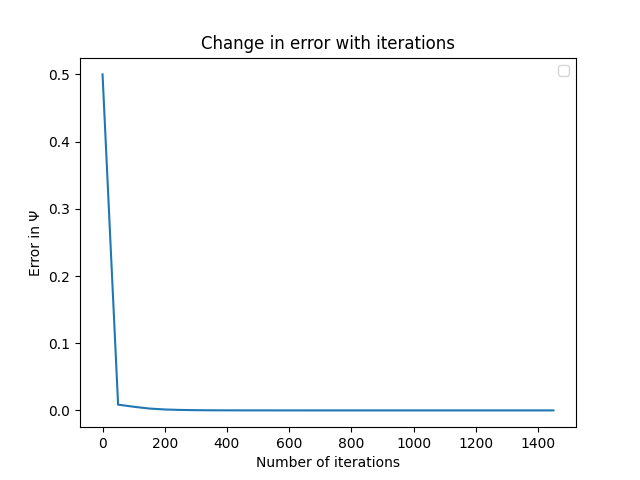
\includegraphics[scale=0.5]{Q2.png} 
    \caption{Error with interations}
   	\label{fig:error)}
   \end{figure}
   
\subsection{Graphing the results}
Its time to analyse how error evolves through the iterations. Anytime we have something like an exponential, we should extract the exponent. However,
it is an exponential decay only for larger iteration numbers. Let us try to fit the entire vector and only the
portion beyond 500. errors decay exponentially in the form 
$$y=Ae^{Bx}$$ after taking log, $$\log{y}=\log{A}+Bx$$. On the semilog plot the errors look like a straight line, which justifies this hunch. $y$ is the error for the $x^{th}$ iteration.  To extract the fit, we need A and B. This is done using our good old \texttt{lstsq}. 
\begin{verbatim}
x_fit = np.zeros((Niter, 2))
x_fit[:,0] = list(range(1, Niter+1))
x_fit[:, 1] = 1
(B, A) = np.linalg.lstsq(x_fit, np.log(errors))[0]
A = np.exp(A)
semilogy(range(Niter)[::50],A*(np.exp(B * range(Niter)))[::50],
 'ro-', label='fit1 = entire error vector')

\end{verbatim} 
The \texttt{lstsq} line returns two data; \texttt{x\_fit} and a $\log$ of \texttt{errors} is passed to it. Based on this the function returns the closest fit - the numerical values of $\log{A}$ and $B$.  Then I plot the hence obtained fit (this is $fit1$), taking every $50^{th}$ value. 

I also plot the same fit again, but this time, for error numbers after the $500^{th}$ iteration. This is $fit2$ can be observed in the legend of Figure 4. The originally obtained errors are also graphed in the same space. 

   \begin{figure}[!tbh]
   	\centering
  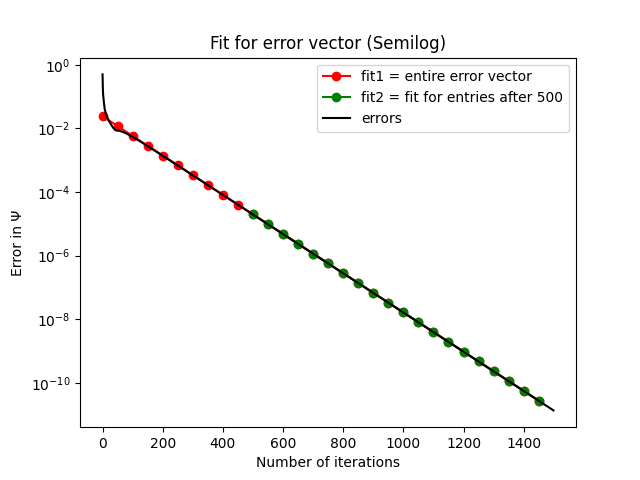
\includegraphics[scale=0.5]{Q3.png} 
    \caption{Error Fitting}
   	\label{fig:error fitting)}
   \end{figure}
   
Notice the magnitude of error - the order is $10^{-4}$ at 400 iterations and keeps going down. This is the precision \texttt{lstsq} has. The difference might not be clear here in Figure 4 as the three lines look overlapping. So Figure 5 provides a closer look. 

\begin{figure}[!tbh]
   	\centering
  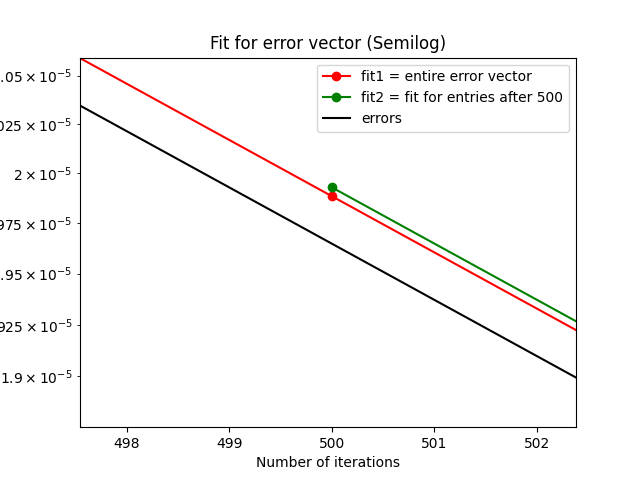
\includegraphics[scale=0.5]{closerlook.png} 
    \caption{Error Fitting: A Closer Look}
   	\label{fig:error fitting 2)}
   \end{figure}
   
All good? Not yet. There's a catch. \texttt{lstsq} is so nice that it drives error to zero after certain number of iterations. In the same parameters I played with so far, if I increase \texttt{Niter} to 3000, what I got is in Figure 6. 

\begin{figure}[!tbh]
   	\centering
  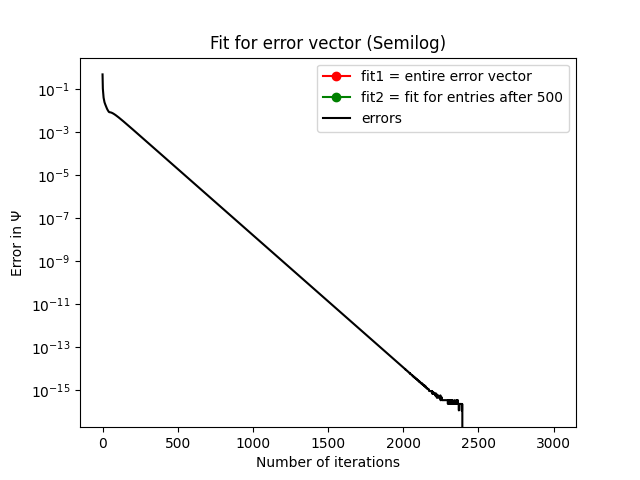
\includegraphics[scale=0.5]{zeroerror.png} 
    \caption{Potential Contour Plot}
   	\label{fig:contour potential)}
   \end{figure}
   The reason why fitting didnt work is $\log0$ creeping into the calculations. So to mitigate this issue, I used another loop that stops calculating error after getting the zero and plots accordingly. This is done by the following code
\begin{verbatim}
for i in range(Niter):
    if errors[i] == 0:
        (B, A) = np.linalg.lstsq(x_fit[:i,:], np.log
          (errors[:i]))[0]
        A = np.exp(A)
        semilogy(range(i)[::50], A*(np.exp(B*range(i)))[::50],
         'ro-', label='fit1 = 
         entire error vector when error vanishes')
        semilogy(range(i), errors[:i], 'black', label='errors')
        xlabel("Number of iterations")
        ylabel("Error in \u03A8")
        title("Fit for error vector (Semilog) when error vanishes")
        legend()
        show()
        break
\end{verbatim}

For 3000 iterations the result is now in Figure 7.

\begin{figure}[!tbh]
   	\centering
  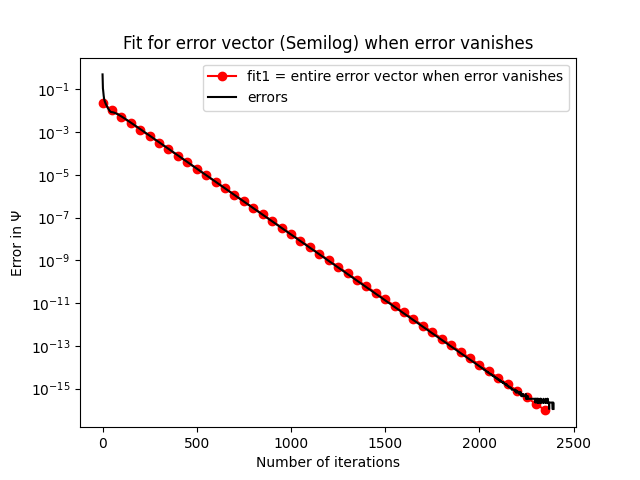
\includegraphics[scale=0.5]{errorcorrected.png} 
    \caption{Error Fitting (Adjusted)}
   	\label{fig:adjusted fitting}
   \end{figure}
  
\subsection{Surface Plot of Potential}
This is a 3D plot. Setting a \texttt{stride} to zero causes the data to be not sampled in the corresponding direction, producing a 3D line plot rather than a wireframe plot; so we set it to 1. Figure 8 shows the plot.

\begin{verbatim}
fig1=figure(4) # open a new figure
ax=p3.Axes3D(fig1) # Axes3D is the means to do a surface plot
surf = ax.plot_surface(X, Y, phi, rstride=1,
 cstride=1, cmap=cm.jet, label='Potential')
xlabel(r'x $\rightarrow$')
ylabel(r'y $\rightarrow$')
title('The 3-D surface plot of the potential')
show()
\end{verbatim}

\begin{figure}[!tbh]
   	\centering
  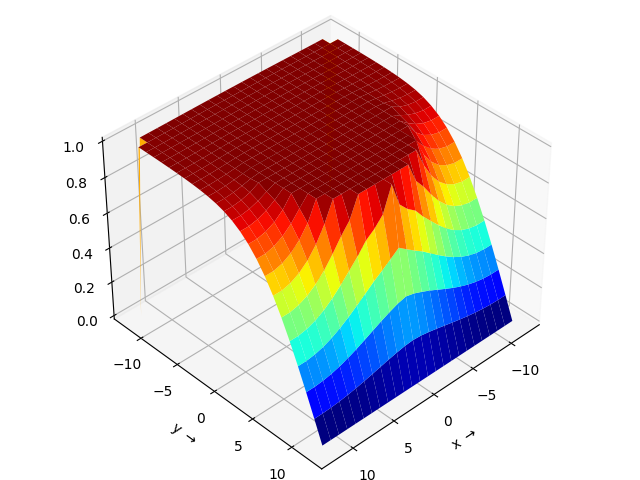
\includegraphics[scale=0.5]{Q4.png} 
    \caption{Surface Plot Of Potential}
   	\label{fig:surface plot potential)}
   \end{figure}
   
\subsection{Contour Plot Of Potential}
Figure 2 had the potential contours when we just initialised the matrix and only had the central 1 V coordinates. Now that I have updated potential of each point to great accuracy, its time to see what I've got finally (in 2D). Using the \texttt{contourf} function again, marking 1 V points in red, I get Figure 9. 

\begin{figure}[!tbh]
   	\centering
  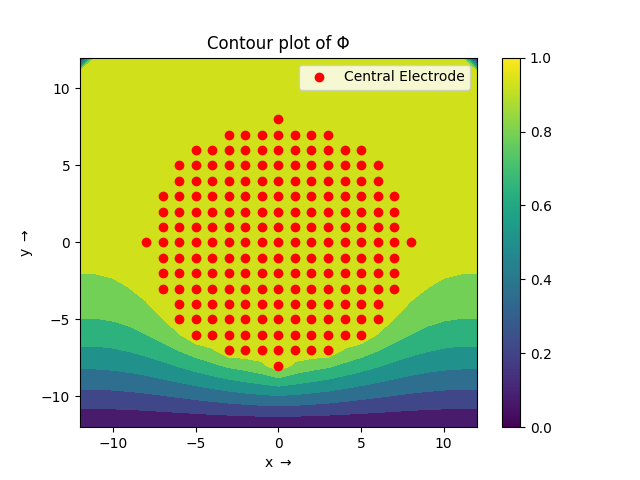
\includegraphics[scale=0.5]{Q5.png} 
    \caption{Potential Contour Plot Final}
   	\label{fig:contour potential final)}
   \end{figure} 
   
\subsection{Vector Plot Of Currents}
 Current is proportional to Electric Field and hence, (ignoring constants) $\nabla \phi$.
$$j_x = -{\partial \phi}/{\partial x}$$
$$j_y = -\partial\phi/\partial y$$
This numerically translates to 
$$J_{x,ij} = \frac{1}{2}(\phi_{i,j-1}-\phi_{i,j+1})$$
$$J_{y,ij} = \frac{1}{2}(\phi_{i-1,j}-\phi_{i+1,j})$$

Now I create arrays \texttt{Jx} and \texttt{Jy}. The \texttt{quiver} function plots the vector plot - Figure 10.

\begin{verbatim}
Jx = np.zeros((Ny, Nx))  
# since x current along parallel sides is 0
Jx[:, 1:-1] = (phi[:, :-2] - phi[:, 2:])/2

Jy = np.zeros((Ny, Nx))  
# since y current along top and bottom sides is 0
Jy[1:-1, :] = (phi[:-2, :] - phi[2:, :])/2

quiver(x, y, -Jx[::-1, :], -Jy[::-1, :], scale=5)
scatter(X[ii], Y[ii], c='r', marker='o',
 label='Central Electrode')
legend()
xlabel(r'x $\rightarrow$')
ylabel(r'y $\rightarrow$')
title("The Vector Plot of the Current Flow")
show()
\end{verbatim}

\begin{figure}[!tbh]
   	\centering
  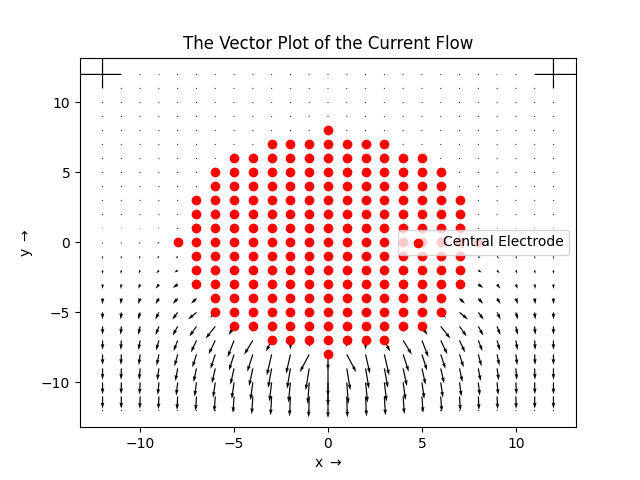
\includegraphics[scale=0.5]{Q6.png} 
    \caption{Vector Plot of Current}
   	\label{fig:vector plot)}
   \end{figure}

Much current doesn't flow in the top part because of symmetry and the fact that the electrode is at the center and the potential gradient is towards the bottom. There will definitely not be a normal component of current up there. Say if there was a parallel component, an equal and opposite current would cancel it out, thanks to the symmetry. Most of the current is in the narrow region at the bottom. That is what will get strongly heated.
  

\section{Conclusion}
 The aim that I took at the beginning of this report is now seen to have been accomplished. I analysed the potential at various points on a 2-dimensional copper plate for the given arrangement. Towards the end I saw how currents are established in the plate. The contour and 3D plots give a deeper insight into what it really looks like. The amazing part of the entire algorithm was vectorized code which did a lot in very few lines.


\end{document}



 